

\documentclass{article}
\usepackage[utf8]{inputenc}
\usepackage{authblk}
\usepackage{setspace}
\usepackage[margin=1.25in]{geometry}
\usepackage{graphicx}
\graphicspath{ {./figures/} }
\usepackage{subcaption}
\usepackage{amsmath}
\usepackage{lineno}
\linenumbers


%%%%%% Bibliography %%%%%%
% Replace "sample" in the \addbibresource line below with the name of your .bib file.
\usepackage[style=nejm, 
citestyle=numeric-comp,
sorting=none]{biblatex}
\addbibresource{sample.bib}

%%%%%% Title %%%%%%
% Full titles can be a maximum of 200 characters, including spaces. 
% Title Format: Use title case, capitalizing the first letter of each word, except for certain small words, such as articles and short prepositions
\title{Master's timeline}

%%%%%% Authors %%%%%%
% Authors should be listed in order of contribution to the paper, by full first name, then middle initial (if any), followed by last name and separated by commas.
% Please do not use initials for first names. If you use your middle name as a full name, use an initial for the first name and spell out your full middle name.
% Use a superscript asterisk (*) to identify the corresponding author and be sure to include that person’s e-mail address. Use symbols (in this order: †, ‡, §, ||, ¶, #, ††, ‡‡, etc.) for author notes, such as present addresses, “These authors contributed equally to this work” notations, and similar information.
% You can include group authors, but please include a list of the actual authors (the group members) in the Supplementary Materials.
\author[]{Christophe Rouleau-Desrochers}


%%%%%% Affiliations %%%%%%
%%%%%% Date %%%%%%
% Date is optional
\date{19 September, 2024 \\ (started on the plane from Edmonton to Montreal)}

%%%%%% Spacing %%%%%%
% Use paragraph spacing of 1.5 or 2 (for double spacing, use command \doublespacing)

\onehalfspacing

\begin{document}

\maketitle

%%%%%% 2024 %%%%%%
\section{2024}
\subsection {Autumn}
\begin {itemize}
	\item Fuelinex: senescence data collection
	\item Fuelinex: literature review
	\item Award applications and specifically CGSM
	\item Class 1: Biomathematics
	\item Side project planning
	\item Dendrometers troubleshooting
	\item Form committee
\end {itemize}

%%%%%% 2025 %%%%%%
\section {2025}
\subsection {Winter}
\begin {itemize}
	\item Fuelinex: tree repotting
	\item Fuelinex: diameter and height data collection
	\item Class 2: Lizzie's bayesian class
	\item Class 3: Dolph's quantitative methods class (unconfirmed)
	\item Start side project
	\item First committee meeting
\end {itemize}

\subsection {Summer}
\begin {itemize}
	\item Fuelinex: bud burst and shoot elongation
	\item Fuelinex: start analysis
\end {itemize}

\subsection {Autumn}
\begin {itemize}
	\item Fuelinex: biomass data collection
	\item Fuelinex: tree rings analysis 
	\item Start writting thesis 
	\item Class 4: last class (TBD)
	\item Semester abroad (??)
\end {itemize}

%%%%%% 2026 %%%%%%
\section {2026}
\subsection {Winter}
\begin {itemize}
	\item Finish writting thesis
	\item Finish analysis
	\item Submit first draft
\end {itemize}

\subsection {Summer}
\begin {itemize}
	\item Thesis defense
\end {itemize}

%%%%%%

%%%%%\subsection{Experimental Design}
%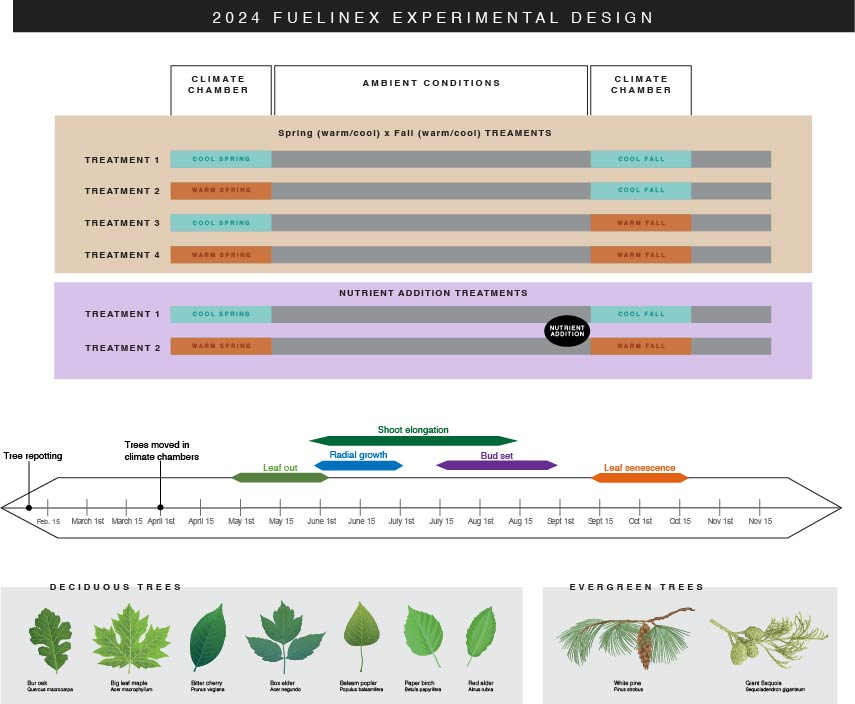
\includegraphics[]{../experimental_design/Fuelinex_Design_V4.jpg}

\end{document}
